\clearpage







\section{Abstract}


\subsubsection{One or two sentences providing a basic introduction to the field}
% comprehensible to a scientist in any discipline.



\subsubsection{Two to three sentences of more detailed background}
% comprehensible to scientists in related disciplines.


\subsubsection{One sentence clearly stating the general problem (the gap)}
% being addressed by this particular study.


\subsubsection{One sentence summarising the main result}
%  (with the words “here we show” or their equivalent).


\subsubsection{Two or three sentences explaining what the main result reveals in direct comparison to what was thought to be the case previously}
% or how the main result adds to previous knowledge


\subsubsection{One or two sentences to put the results into a more general context.}



\subsubsection{Two or three sentences to provide a broader perspective, }
% readily comprehensible to a scientist in any discipline.



%%%%%%%%%%%%%%%%%%%%%%%%%%%%%%%%%%%%%%%%%%%%%%%%%%%%%%%%%%%%%%%%%%%%%%%%%%%%%%%%%%%%%%%%%%%%%%%%%%%%%%%%%%%%%%%%%%%%%%%%%%%%%%%%%%%%%%%%%%%%%%%%%%%%%%%%%%%

\clearpage
\section{Introduction}

%%%%%%%%%%%%%%%%%%%%%%%%%%%%%%%%%%%%%%%%%%%%%%%%%%%%%%%%%%%%%%%%%%%%%%%%%%%%%%%%%%%%%%%%%%%%%%%%%%%%%%%%%%%%%%%%%%%%%%%%%%%%%%%%%%%%%%%%%%%%%%%%%%%%%%%%%%%





%%%%%%%%%%%%%%%%%%%%%%%%%%%%%%%%%%%%%%%%%%%%%%%%%%%%%%%%%%%%%%%%%%%%%%%%%%%%%%%%%%%%%%%%%%%%%%%%%%%%%%%%%%%%%%%%%%%%%%%%%%%%%%%%%%%%%%%%%%%%%%%%%%%%%%%%%%%

\clearpage
\section{Methods}

%%%%%%%%%%%%%%%%%%%%%%%%%%%%%%%%%%%%%%%%%%%%%%%%%%%%%%%%%%%%%%%%%%%%%%%%%%%%%%%%%%%%%%%%%%%%%%%%%%%%%%%%%%%%%%%%%%%%%%%%%%%%%%%%%%%%%%%%%%%%%%%%%%%%%%%%%%%

To measure pathogen richness I used data from \cite{luis2013comparison}. 
These simply include known infections of a bat species with a pathogen species. 
Only species with at least one pathogen were included in the analysis.
To control for study bias I collected the number of pubmed and scholar citations for each bat species including synonyms from ITIS \cite{itis} via the taxize package \cite{chamberlain2013taxize}.
The counts were scraped using the rvest package \cite{rvest}.






I used two measures of population structure. 
$F_{ST}$ and the number of subspecies.
The number of of subspecies was counted using the Wilson and Reeder taxonomy \cite{wilson2005mammal}.

\begin{knitrout}\footnotesize
\definecolor{shadecolor}{rgb}{0.137, 0.137, 0.137}\color{fgcolor}\begin{figure}[t]

{\centering 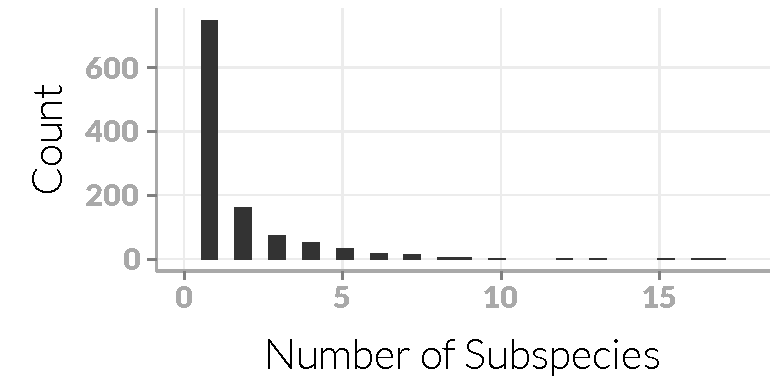
\includegraphics[width=0.8\textwidth]{figure/wilsonReaderTaxonomyRead-1} 

}

\caption[Histogram of number of subspecies]{Histogram of number of subspecies}\label{fig:wilsonReaderTaxonomyRead}
\end{figure}


\end{knitrout}

\begin{knitrout}\footnotesize
\definecolor{shadecolor}{rgb}{0.137, 0.137, 0.137}\color{fgcolor}\begin{figure}[t]

{\centering 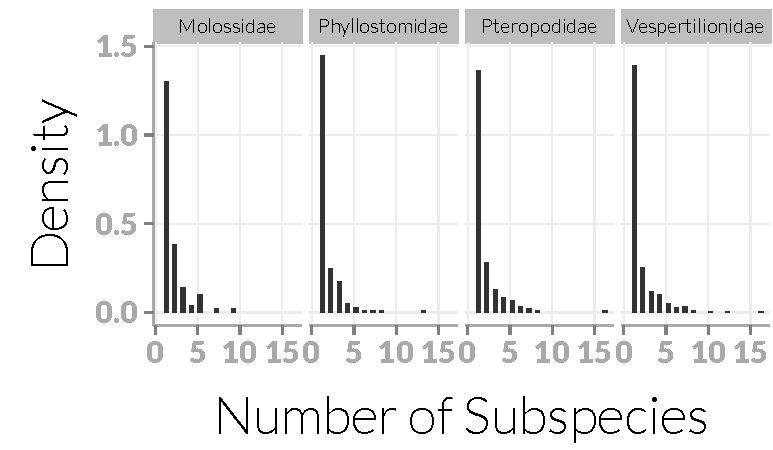
\includegraphics[width=0.8\textwidth]{figure/subsHistsByFam-1} 

}

\caption[Histograms of number of subspecies for the families with many species]{Histograms of number of subspecies for the families with many species.}\label{fig:subsHistsByFam}
\end{figure}


\end{knitrout}



\begin{knitrout}\footnotesize
\definecolor{shadecolor}{rgb}{0.137, 0.137, 0.137}\color{fgcolor}\begin{figure}[t]

{\centering 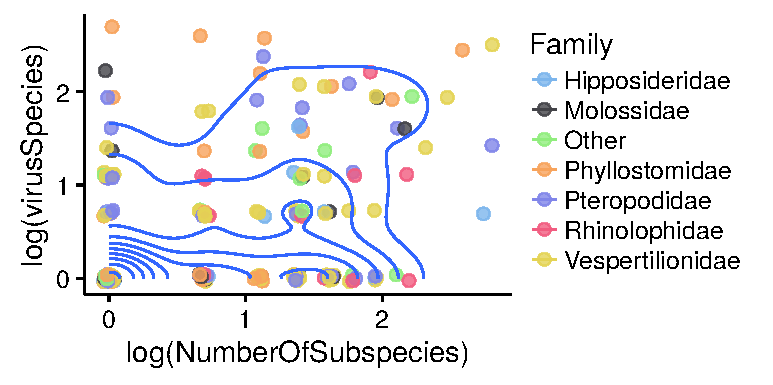
\includegraphics[width=\textwidth]{figure/subsDataFrame-1} 

}

\caption[Number of viruses against number of subspecies.]{
Number of viruses against number of subspecies.
Points are coloured by family, with families with less than 10 species being grouped into "other".
Contours show the 2D density of points and suggest a positive correlation.
}\label{fig:subsDataFrame}
\end{figure}


\end{knitrout}

\begin{knitrout}\footnotesize
\definecolor{shadecolor}{rgb}{0.137, 0.137, 0.137}\color{fgcolor}\begin{figure}[t]

{\centering 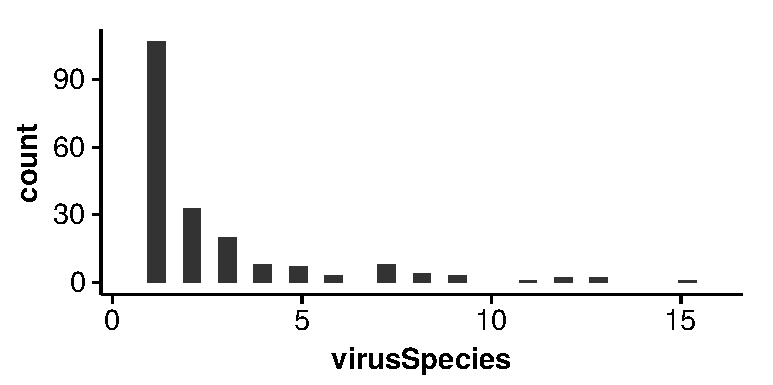
\includegraphics[width=0.8\textwidth]{figure/virusHist-1} 

}

\caption[Histogram of known viruses per species]{Histogram of known viruses per species}\label{fig:virusHist}
\end{figure}


\end{knitrout}



Measures of body mass are taken from Pantheria \cite{jones2009pantheria}.
They are log transformed due to the strong right skew.
























\begin{knitrout}\footnotesize
\definecolor{shadecolor}{rgb}{0.137, 0.137, 0.137}\color{fgcolor}\begin{figure}[t]

{\centering 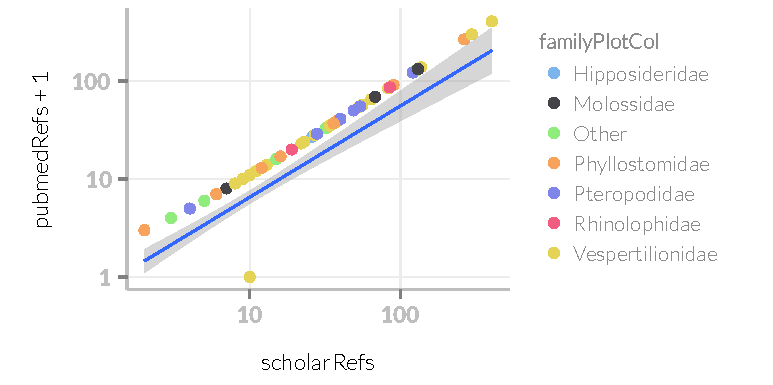
\includegraphics[width=0.8\textwidth]{figure/scholarvspubmed-1} 

}

\caption[Logged number of references on scholar and pubmed, with a fitted (unphylogenetic) linear model]{Logged number of references on scholar and pubmed, with a fitted (unphylogenetic) linear model. Colours indicate family.}\label{fig:scholarvspubmed}
\end{figure}


\end{knitrout}




%Pubmed was scraped on pubmedScrapeDate and Google Scholar was scraped on scholarScrapeDate

To control for phylogenetic nonindependance I used the best-supported phylogeny from \cite{fritz2009geographical} which is the supertree from \cite{bininda2007delayed} with names updated to match the Wilson \& Reeder taxonomy \cite{wilson2005mammal}.
Phylogenetic manipulation was performed using the ape package \cite{ape}.




\begin{knitrout}\footnotesize
\definecolor{shadecolor}{rgb}{0.137, 0.137, 0.137}\color{fgcolor}\begin{figure}[t]

{\centering 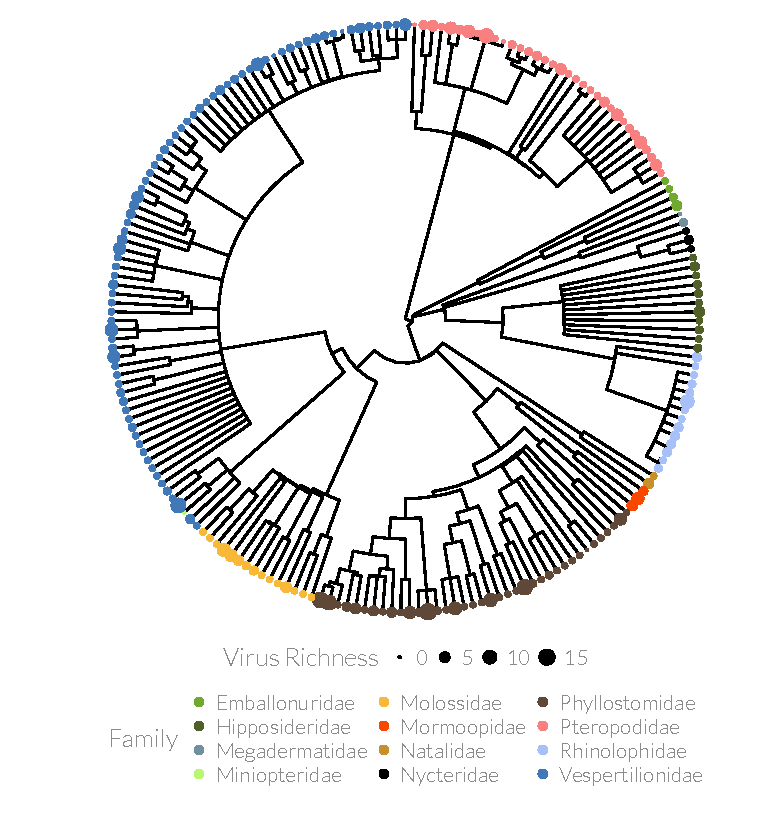
\includegraphics[width=0.8\textwidth]{figure/treePlot-1} 

}

\caption[Pruned phylogeny with dot size showing number of pathogens and colour showing family]{Pruned phylogeny with dot size showing number of pathogens and colour showing family.}\label{fig:treePlot}
\end{figure}


\end{knitrout}



\begin{knitrout}\footnotesize
\definecolor{shadecolor}{rgb}{0.137, 0.137, 0.137}\color{fgcolor}\begin{figure}[t]

{\centering 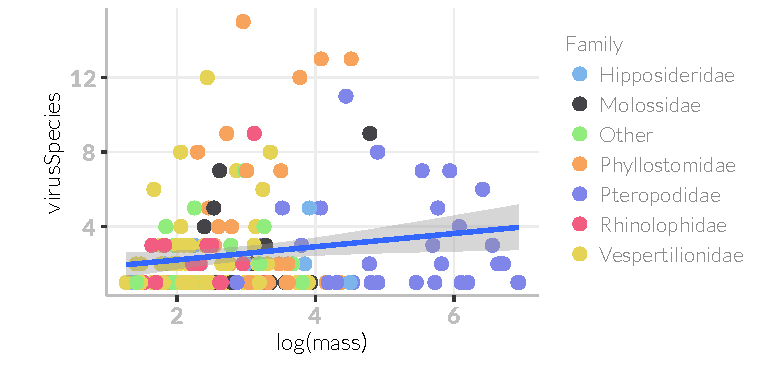
\includegraphics[width=0.8\textwidth]{figure/subsDataviz-1} 

}

\caption[Unlogged number of virus species against log mass with a non-phylogenetic linear model added]{Unlogged number of virus species against log mass with a non-phylogenetic linear model added. Points are significantly jittered to try and reveal the sever overplotting in the bottom left corner in particular.}\label{fig:subsDataviz}
\end{figure}

\begin{figure}[t]

{\centering 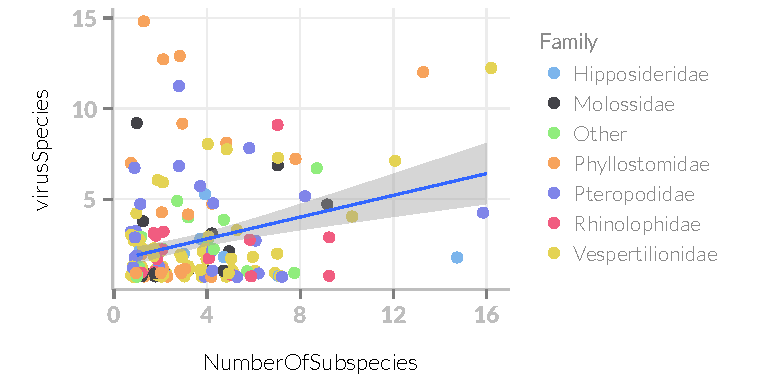
\includegraphics[width=0.8\textwidth]{figure/subsDataviz-2} 

}

\caption[Number of virus species against logged number of subspecies (not marginal) with a non-phylogenetic linear model added]{Number of virus species against logged number of subspecies (not marginal) with a non-phylogenetic linear model added. Points are significantly jittered to try and reveal the sever overplotting in the bottom left corner in particular.}\label{fig:subsDataviz}
\end{figure}

\begin{figure}[t]

{\centering 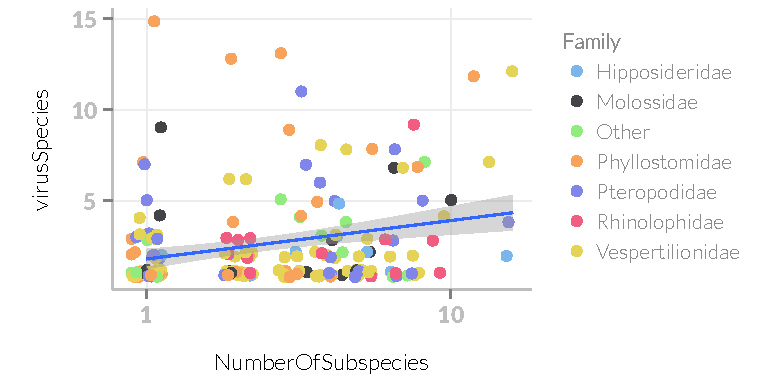
\includegraphics[width=0.8\textwidth]{figure/subsDataviz-3} 

}

\caption[Number of virus species against logged number of subspecies (not marginal) with a non-phylogenetic linear model added]{Number of virus species against logged number of subspecies (not marginal) with a non-phylogenetic linear model added.}\label{fig:subsDataviz}
\end{figure}

\begin{figure}[t]

{\centering 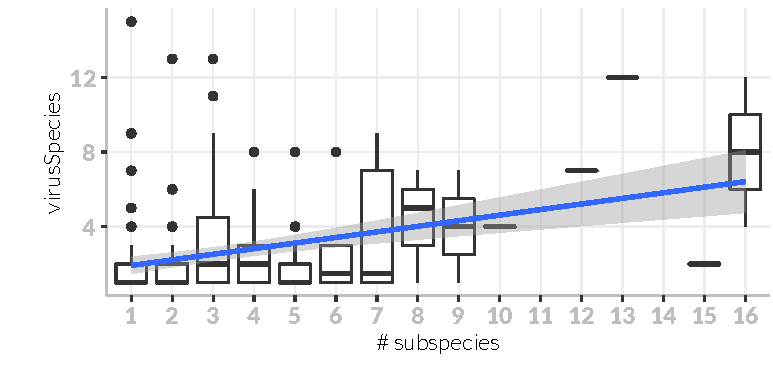
\includegraphics[width=0.8\textwidth]{figure/subsDataviz-4} 

}

\caption[Number of virus species against number of subspecies]{Number of virus species against number of subspecies. Data within a number of subspecies are plotted as boxplots with the dark bar showing the median, the box showing the interquartile range, vertical lines showing the range and outliers shown as seperate points. A non-phylogenetic linear model is shown in blue}\label{fig:subsDataviz}
\end{figure}

\begin{figure}[t]

{\centering 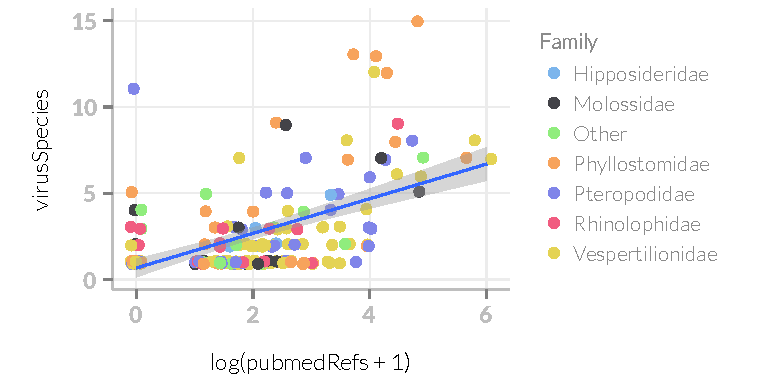
\includegraphics[width=0.8\textwidth]{figure/subsDataviz-5} 

}

\caption[Virus species against study effort (log pubmed references +1)]{Virus species against study effort (log pubmed references +1)}\label{fig:subsDataviz}
\end{figure}


\end{knitrout}


I wanted to run three models using the phylolm package testing the relationship between pathogen richness and log number of subspecies.
I tried phylogenetically controlled, multivariate GLMs with poisson errors and identity links.
This model was fitted both with and without an interaction term between number of subspecies and study effort.
I also fitted a phylogenetically controlled, GLM with poisson errors and identity link to pathogen richness and study effort.
The residuals from this model was then used as the response variable in a multivariate GLM.
However, with these models the numerical optimisation failed to converge.

I ran three models using the caper package \cite{caper} testing the relationship between pathogen richness and log number of subspecies.
All independant variables were log transformed --- study effort was $\log(\text{citations} + 1)$.
I ran phylogenetically controlled, multivariate linear models.
This model was fitted both with and without an interaction term between number of subspecies and study effort.
We also fitted a phylogenetically controlled, GLM with poisson errors and identity link to pathogen richness and study effort.
The residuals from this model was then used as the response variable in a multivariate GLM.



\begin{knitrout}\footnotesize
\definecolor{shadecolor}{rgb}{0.137, 0.137, 0.137}\color{fgcolor}\begin{figure}[t]

{\centering 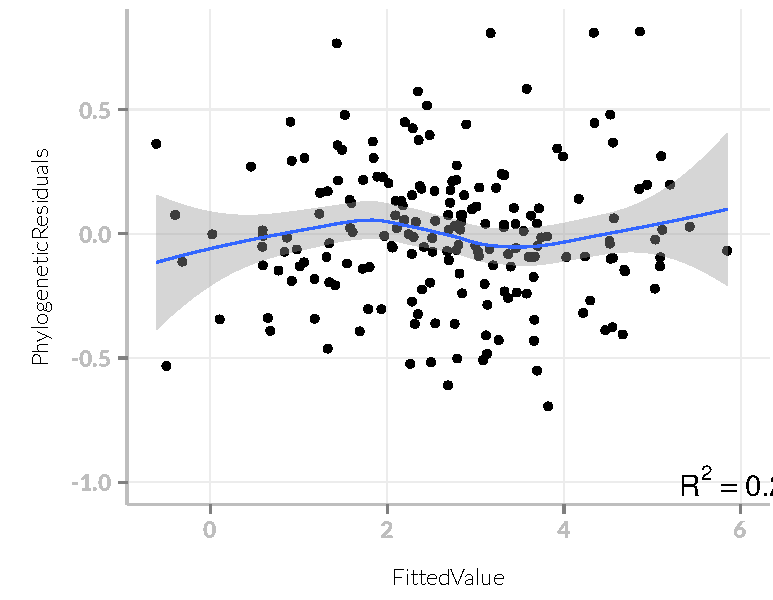
\includegraphics[width=0.8\textwidth]{figure/subsAnalysis-1} 

}

\caption[Fitted values against residuals from the full phylogenetic model (virusSpecies ]{Fitted values against residuals from the full phylogenetic model (virusSpecies $\sim$ log(pubmedRefs + 1) + log(NumberOfSubspecies) +  log(mass)). A loess curve is shown in blue. 
The $R^2$ value give is for the full model (not the loess curve).}\label{fig:subsAnalysis}
\end{figure}

\begin{figure}[t]

{\centering 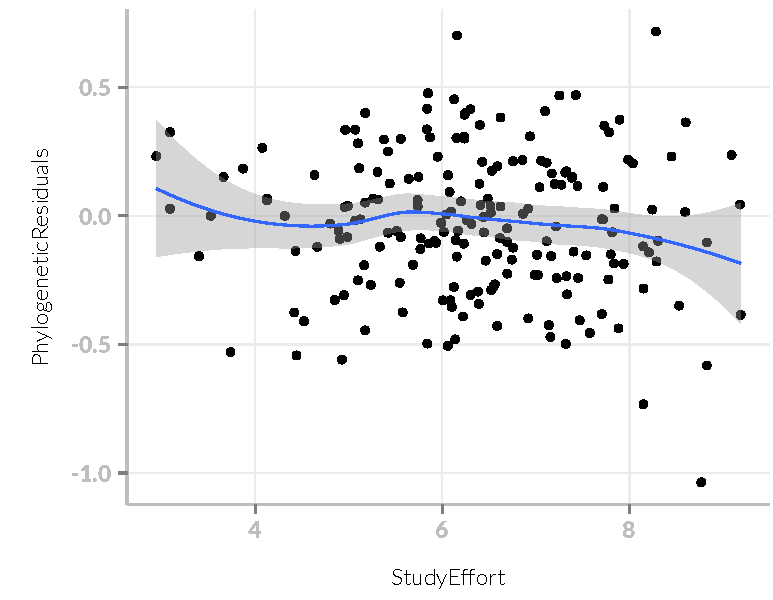
\includegraphics[width=0.8\textwidth]{figure/subsAnalysis-2} 

}

\caption[Study effort against residuals with a loess trend]{Study effort against residuals with a loess trend.}\label{fig:subsAnalysis}
\end{figure}

\begin{figure}[t]

{\centering 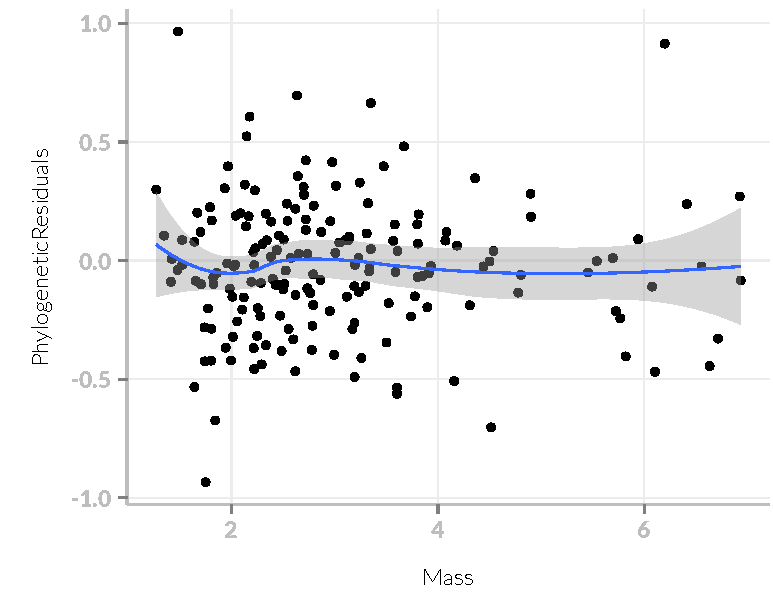
\includegraphics[width=0.8\textwidth]{figure/subsAnalysis-3} 

}

\caption[Mass against residuals with a loess trend shown in blue]{Mass against residuals with a loess trend shown in blue.}\label{fig:subsAnalysis}
\end{figure}

\begin{figure}[t]

{\centering 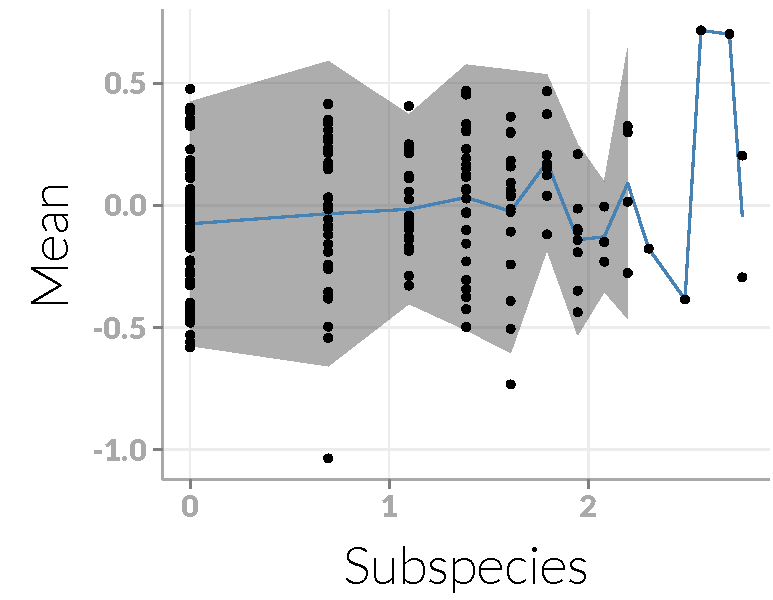
\includegraphics[width=0.8\textwidth]{figure/subsAnalysis-4} 

}

\caption[Logged number of subspecies against phylogenetic residuals]{Logged number of subspecies against phylogenetic residuals. The mean for each value of logged subspecies is shown in blue. A ribbon showing the mean $\pm 1.96{SD}$ is shown in grey. The ribbon does not cover the full range of the x axis as there are not enough data points to calculate the SD towards the right.}\label{fig:subsAnalysis}
\end{figure}

\begin{figure}[t]

{\centering 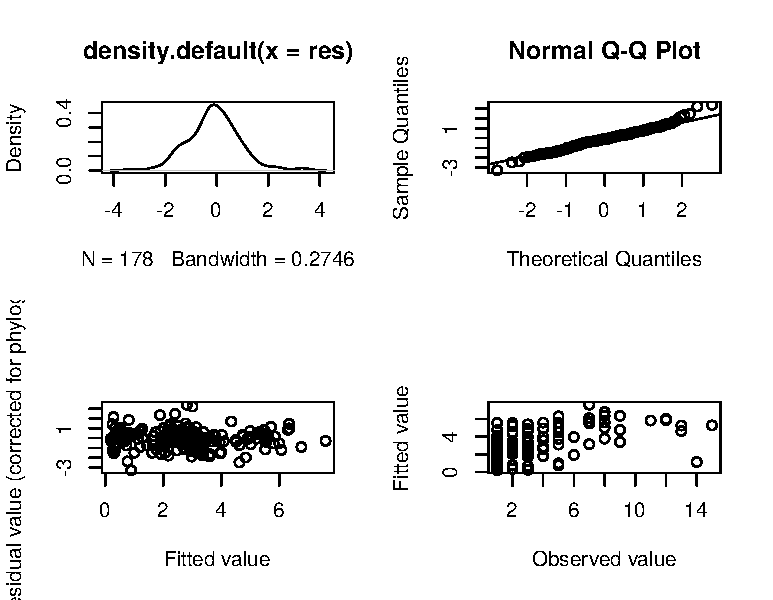
\includegraphics[width=0.8\textwidth]{figure/subsAnalysis-5} 

}

\caption[Fitted values against residuals from the full phylogenetic model (virusSpecies ]{Fitted values against residuals from the full phylogenetic model (virusSpecies $\sim$ NumberOfSubspecies + log(pubmedRefs + 1) +   log(mass)). A loess curve is shown in blue.
The $R^2$ value give is for the full model (not the loess curve).}\label{fig:subsAnalysis}
\end{figure}

\begin{figure}[t]

{\centering 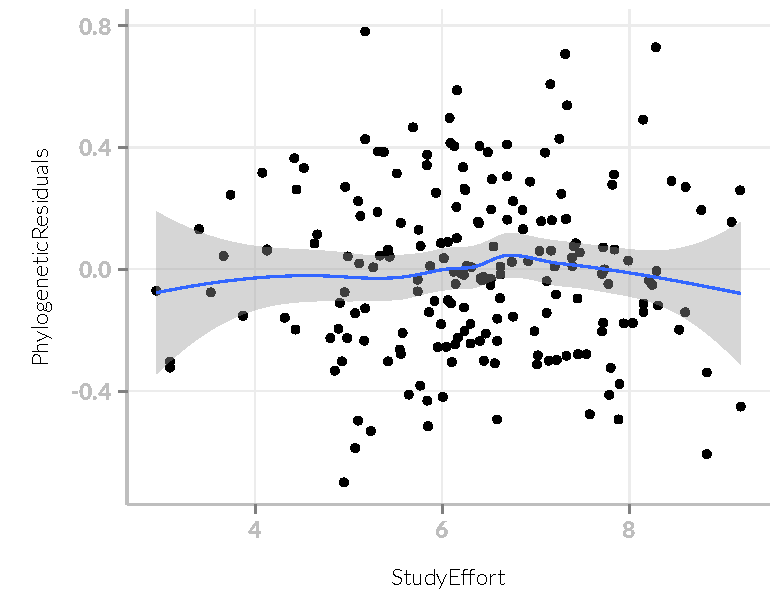
\includegraphics[width=0.8\textwidth]{figure/subsAnalysis-6} 

}

\caption[Study effort against residuals (unlogged subspecies) with a loess trend]{Study effort against residuals (unlogged subspecies) with a loess trend.}\label{fig:subsAnalysis}
\end{figure}

\begin{figure}[t]

{\centering 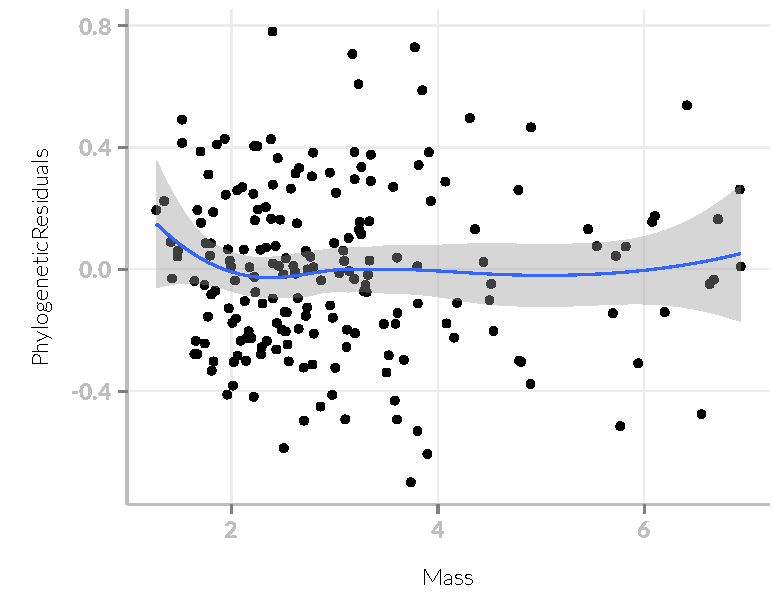
\includegraphics[width=0.8\textwidth]{figure/subsAnalysis-7} 

}

\caption[Mass against residuals  (unlogged subspecies) with a loess trend shown in blue]{Mass against residuals  (unlogged subspecies) with a loess trend shown in blue.}\label{fig:subsAnalysis}
\end{figure}

\begin{figure}[t]

{\centering 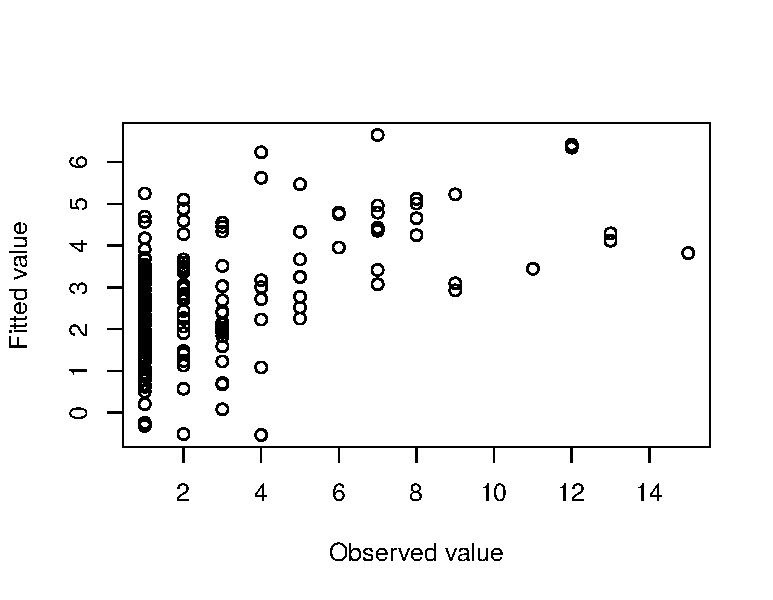
\includegraphics[width=0.8\textwidth]{figure/subsAnalysis-8} 

}

\caption[Number of subspecies against phylogenetic residuals]{Number of subspecies against phylogenetic residuals. The mean for each value of logged subspecies is shown in blue. A ribbon showing the mean $\pm 1.96{SD}$ is shown in grey. The ribbon does not cover the full range of the x axis as there are not enough data points to calculate the SD towards the right.}\label{fig:subsAnalysis}
\end{figure}


\end{knitrout}
\clearpage


\begin{knitrout}\footnotesize
\definecolor{shadecolor}{rgb}{0.137, 0.137, 0.137}\color{fgcolor}\begin{figure}[t]

{\centering 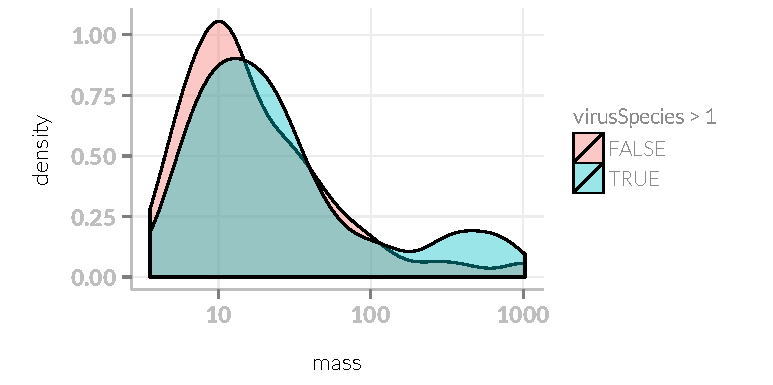
\includegraphics[width=0.8\textwidth]{figure/rm1vir-1} 

}

\caption[Density of mass variable for 1 or >1 viruses.]{
Density curves for mass of bat species with 1 or > 1 pathogen species.
The hump of the \emph{Pteropodidae} (large fruit bats) can be seen.
It seems likely that this family are overstudied as they carry a number of important zoonotics.}\label{fig:rm1vir}
\end{figure}

\begin{figure}[t]

{\centering 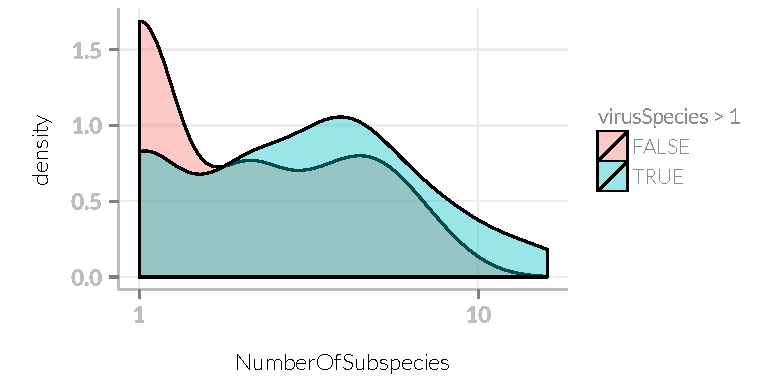
\includegraphics[width=0.8\textwidth]{figure/rm1vir-2} 

}

\caption[Density of number of subspecies 1 or >1 viruses.]{Density curves for number of subspecies of bat species with 1 or > 1 pathogen species.}\label{fig:rm1vir}
\end{figure}

\begin{figure}[t]

{\centering 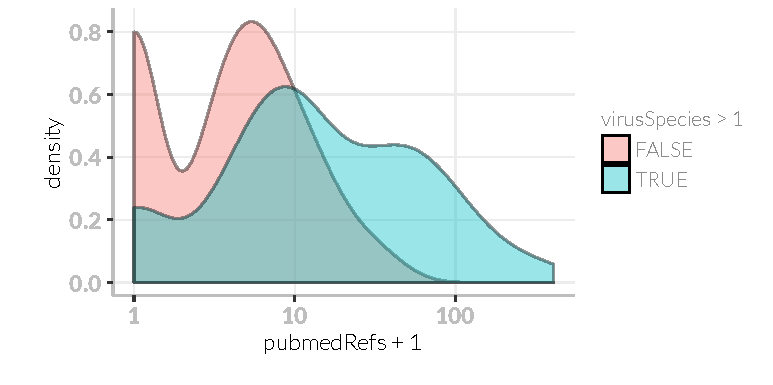
\includegraphics[width=0.8\textwidth]{figure/rm1vir-3} 

}

\caption[Density of number of pubmed references 1 or >1 viruses.]{Density curves for number of pubmed references of bat species with 1 or > 1 pathogen species.
There is a clear trend that many species with only 1 virus species, have 0 pubmed references.
}\label{fig:rm1vir}
\end{figure}

\begin{figure}[t]

{\centering 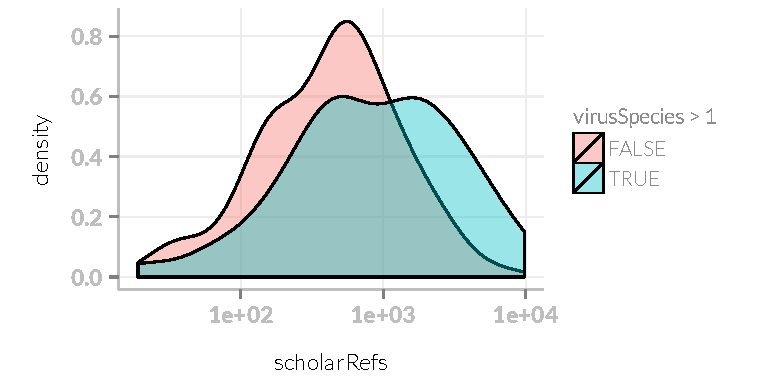
\includegraphics[width=0.8\textwidth]{figure/rm1vir-4} 

}

\caption[Density of number of scholar references 1 or >1 viruses.]{Density curves for number of scholar references of bat species with 1 or > 1 pathogen species.
The strong trend in the pubmed data is not noticeable here.
}\label{fig:rm1vir}
\end{figure}


\end{knitrout}

\clearpage
\begin{knitrout}\footnotesize
\definecolor{shadecolor}{rgb}{0.137, 0.137, 0.137}\color{fgcolor}\begin{figure}[t]

{\centering 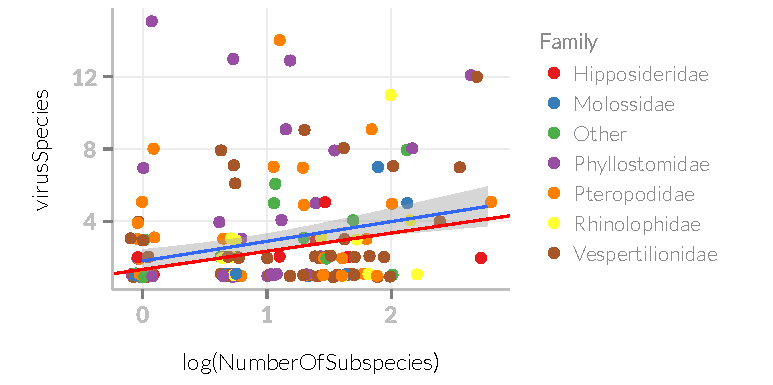
\includegraphics[width=0.8\textwidth]{figure/plotSubspecies-1} 

}

\caption[Number of virus species against log number of subspecies]{Number of virus species against log number of subspecies. Nonphylogenetic trend line in blue. Phylogenetic model (evaluated at mean body mass and mean study effort values) is shown in red.}\label{fig:plotSubspecies}
\end{figure}


\end{knitrout}

\begin{knitrout}\footnotesize
\definecolor{shadecolor}{rgb}{0.137, 0.137, 0.137}\color{fgcolor}\begin{figure}[t]

{\centering 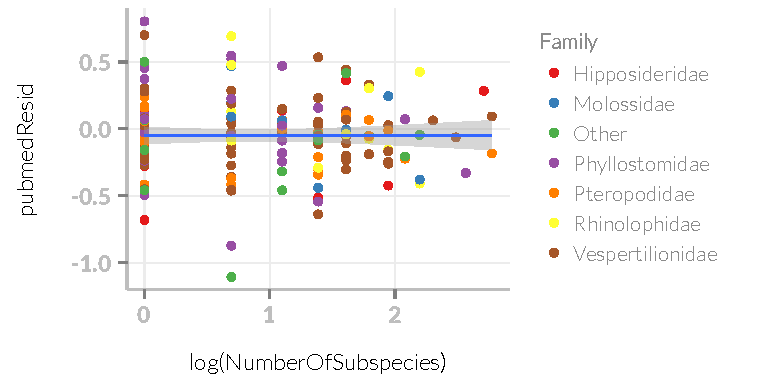
\includegraphics[width=0.8\textwidth]{figure/pubmedresidPlot-1} 

}

\caption[Plot using residuals from number of viruses against number of citations (study effort)]{Plot using residuals from number of viruses against number of citations (study effort). Nonphylogenetic trend line added. }\label{fig:pubmedresidPlot}
\end{figure}


\end{knitrout}

%%%%%%%%%%%%%%%%%%%%%%%%%%%%%%%%%%%%%%%%%%%%%%%%%%%%%%%%%%%%%%%%%%%%%%%%%%%%%%%%%%%%%%%%%%%%%%%%%%%%%%%%%%%%%%%%%%%%%%%%%%%%%%%%%%%%%%%%%%%%%%%%%%%%%%%%%%%

\clearpage
\section{Results}

%%%%%%%%%%%%%%%%%%%%%%%%%%%%%%%%%%%%%%%%%%%%%%%%%%%%%%%%%%%%%%%%%%%%%%%%%%%%%%%%%%%%%%%%%%%%%%%%%%%%%%%%%%%%%%%%%%%%%%%%%%%%%%%%%%%%%%%%%%%%%%%%%%%%%%%%%%%

See Figure \ref{fig:plotSubspeciesCoefs} for a display of estimated coefficients for the two models using number of viruses as the response variable. 
The main model with mass, study effort and number of subspecies as predictors found study effort to be highly significant ($\beta = $1.01, $p = $\ensuremath{3.9\times 10^{-12}}). 
The number of subspecies was marginally significant ($\beta = $ 0.48, $p = $0.06). 
The effect of nonindependance due to phylogeny was very small ($\lambda = $0.07, $p = $0.1).

The interaction term between study effort and number of subspecies, when included, was not significant ($\beta = $ 0.23, $p = $0.12).

The model using the residuals from a regression between number of viruses and study effort as the response variable found no significant affect of number of subspecies. 
Mass was marginally significant.




\begin{knitrout}\footnotesize
\definecolor{shadecolor}{rgb}{0.137, 0.137, 0.137}\color{fgcolor}\begin{figure}[t]

{\centering 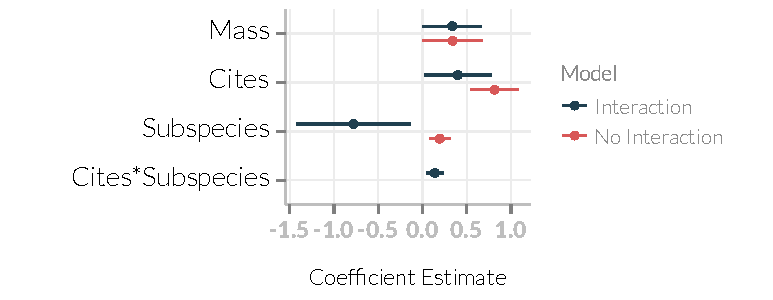
\includegraphics[width=0.8\textwidth]{figure/plotSubspeciesCoefs-1} 

}

\caption[
Plot of coefficient estimates and 95\% confidence intervals for phylogenetic model with (inter) and without (joint) interactions between study effort and number of subspecies]{
Plot of coefficient estimates and 95\% confidence intervals for phylogenetic model with (inter) and without (joint) interactions between study effort and number of subspecies. 
Without interactions, number of subspecies is marginally significant.
}\label{fig:plotSubspeciesCoefs}
\end{figure}


\end{knitrout}










%%%%%%%%%%%%%%%%%%%%%%%%%%%%%%%%%%%%%%%%%%%%%%%%%%%%%%%%%%%%%%%%%%%%%%%%%%%%%%%%%%%%%%%%%%%%%%%%%%%%%%%%%%%%%%%%%%%%%%%%%%%%%%%%%%%%%%%%%%%%%%%%%%%%%%%%%%%

\clearpage
\section{Discussion}  

%%%%%%%%%%%%%%%%%%%%%%%%%%%%%%%%%%%%%%%%%%%%%%%%%%%%%%%%%%%%%%%%%%%%%%%%%%%%%%%%%%%%%%%%%%%%%%%%%%%%%%%%%%%%%%%%%%%%%%%%%%%%%%%%%%%%%%%%%%%%%%%%%%%%%%%%%%%









